\section{Introduction}
\label{sec:introduction}

\todo{Introduction goes here.}

\todo{We motivate the problem of deciding serializability in programmable networks.}

\todo{We talk about some related work if relevant.}

\todo{We show that it's interesting with an example.}

\todo{We describe our main results.}

\todo{Important point: mention the french people here early on, so that the reviewers know that we are aware of them. Also explain clearly what is new here: a tool that can actually run and output certificates.}

\paragraph{Contributions:}
\begin{itemize}
    \item Novel notion of serializability (``atomicity'' or ``semantic serializabillity'') applicable to network systems (\Cref{sec:problem-definition,sec:related:notions-of-serializability})
    \item Decidability results (1 main theorem: \textbf{automatically proving unbounded serializability}, 2 extra theorems: ser=ser decidable, int=int undecidable) (\Cref{sec:formal-results,sec:related:deciding-serializability})
    \item Implementation of decision procedure. Advances in semilinear sets, Petri net reachability heuristics that makes the decision procedure work. (\Cref{sec:implementation,sec:related:petri})
     \item optimizations
     \item case study - real world problems
     \item proof certificate checker
\end{itemize}

\newpage


\subsection{Motivating Example}


Observe the simple program depicted in Listing~\ref{lst:MotivatingExample1Ser}. Each request call \textit{foo} gives rise to a fresh in-flight request. The variable ``X'' is global, and shared among all in-flight requests, while the variable ``y'' is local variable, per each request. 
%
As there are no yields, it is straightforward to see that the program is trivially serializable, with every request \textit{foo}: (i) assigning 1 to the global variable X; (ii) assigning to y to have the value of X, i.e., always 1; (iii) assigning to X the value 0; and (iv) returning the response y. This results to every (request,response) pair to be of the form \textit{(foo, 1)}.
%
The program is slightly altered (in Listing~\ref{lst:MotivatingExample2NonSer}), by adding a yield operation between the aforementioned steps (i) and (ii). Now, by running two \textit{foo} requests that interleave, it is possible to attain a \textit{(foo,0)} request/response pair, which is unattainable in any serial execution of Listing~\ref{lst:MotivatingExample2NonSer} --- as any such serial execution is equivalent to Listing~\ref{lst:MotivatingExample1Ser}, which always responds ``1'' to any request \textit{foo}.


\noindent
\begin{minipage}[t]{0.45\textwidth}
	\begin{minipage}[t]{\textwidth}
		\begin{lstlisting}[caption={Without yield or lock (serializable)},
			label={lst:MotivatingExample1Ser}]
    request foo: 
        X := 1 
        // no yield
        y := X 
        X := 0
        return y 
		\end{lstlisting}
	\end{minipage}
	\vspace{1em}
	\begin{minipage}[t]{\textwidth}
		\begin{lstlisting}[caption={With yield (not serializable)},
			label={lst:MotivatingExample2NonSer}]
    request foo: 
        X := 1 
        yield 
        y := X 
        X := 0
        return y 	
		\end{lstlisting}
	\end{minipage}
\end{minipage}%
\hfill
\begin{minipage}[t]{0.45\textwidth}
	\begin{lstlisting}[caption={With yield and lock (serializable)},
		label={lst:MotivatingExample3Ser}]
    request foo: 
        // lock
        while (L == 1): 
            yield
        L := 1 

        X := 1
        yield
        y := X 
        X := 0

        // unlock    
        L := 0
        return y 
	\end{lstlisting}
\end{minipage}

The program is altered once again in in Listing~\ref{lst:MotivatingExample3Ser}, by adding a fresh global variable ``L'', indicating if the critical section is locked ($L=1$) or not ($L=0$).
By adding a global lock variable, even if an interleaving occurs after yielding, the lock will allow only the first request to terminate, and will then release the lock for the next request. Hence, despite having yields, we attain serializable executions, and only \textit{(foo,1)} request/response pairs are produced, similar to the original program in Listing~\ref{lst:MotivatingExample1Ser}.
%
This simple example demonstrates the motivation for automatic serializability checking, as even small, toy programs can be surprisingly difficult to reason about when assessing their serializable behavior.




%\begin{figure}[H]
%	\centering
%	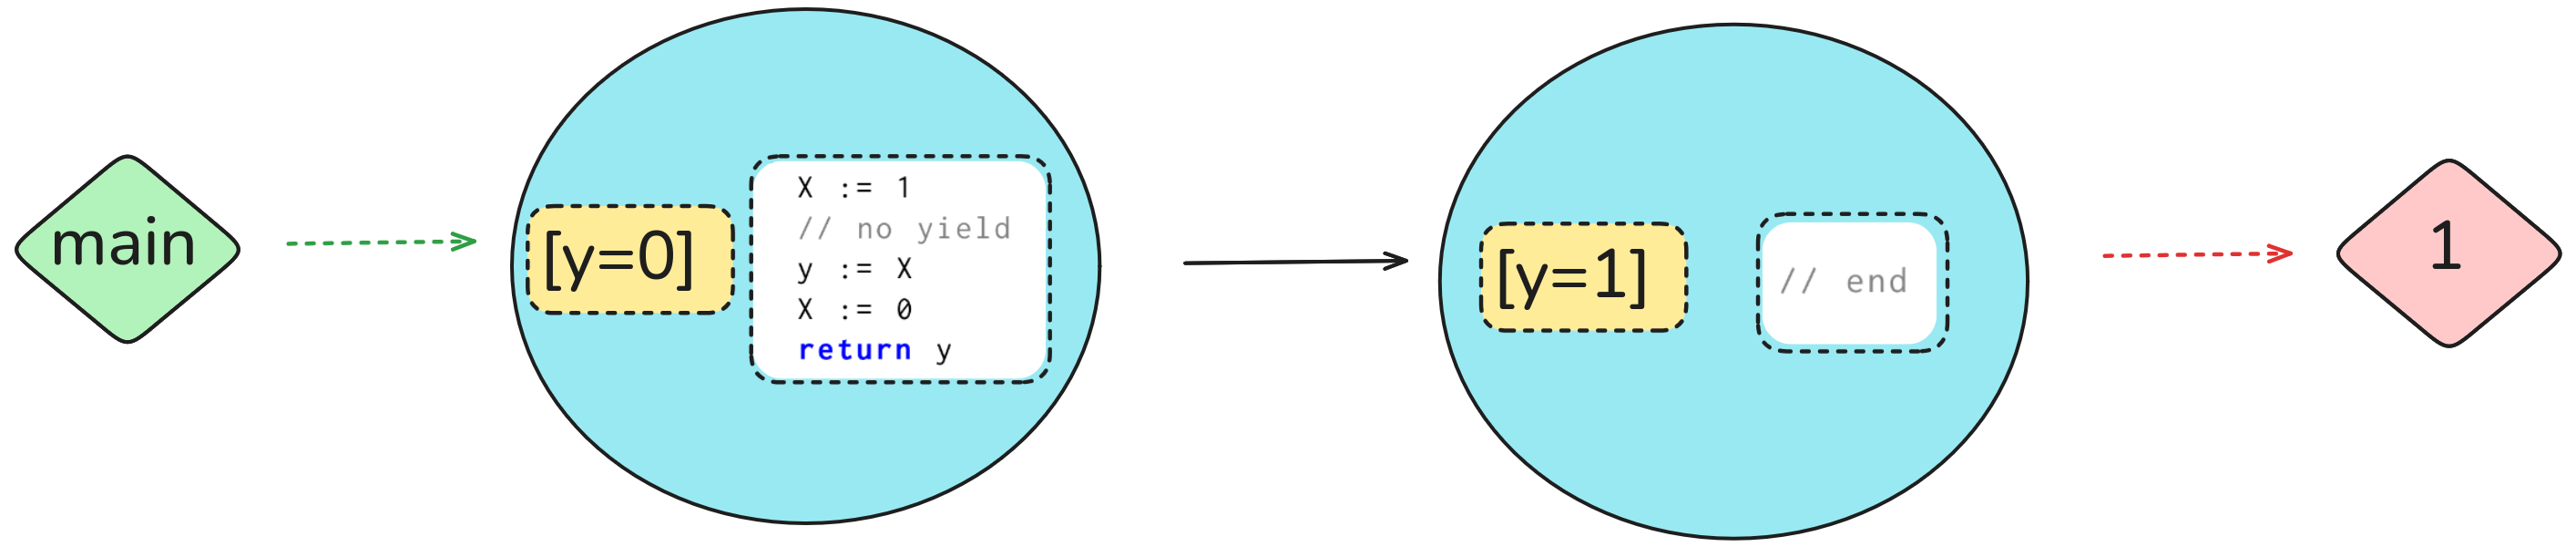
\includegraphics[width=1.0\linewidth]{plots/code_1_ser_NS.png}
%	\caption{Routing policy in example 5.}
%	\label{fig:code1NS}
%\end{figure}

